% Options for packages loaded elsewhere
\PassOptionsToPackage{unicode}{hyperref}
\PassOptionsToPackage{hyphens}{url}
%
\documentclass[
  ignorenonframetext,
]{beamer}
\usepackage{pgfpages}
\setbeamertemplate{caption}[numbered]
\setbeamertemplate{caption label separator}{: }
\setbeamercolor{caption name}{fg=normal text.fg}
\beamertemplatenavigationsymbolsempty
% Prevent slide breaks in the middle of a paragraph
\widowpenalties 1 10000
\raggedbottom
\setbeamertemplate{part page}{
  \centering
  \begin{beamercolorbox}[sep=16pt,center]{part title}
    \usebeamerfont{part title}\insertpart\par
  \end{beamercolorbox}
}
\setbeamertemplate{section page}{
  \centering
  \begin{beamercolorbox}[sep=12pt,center]{part title}
    \usebeamerfont{section title}\insertsection\par
  \end{beamercolorbox}
}
\setbeamertemplate{subsection page}{
  \centering
  \begin{beamercolorbox}[sep=8pt,center]{part title}
    \usebeamerfont{subsection title}\insertsubsection\par
  \end{beamercolorbox}
}
\AtBeginPart{
  \frame{\partpage}
}
\AtBeginSection{
  \ifbibliography
  \else
    \frame{\sectionpage}
  \fi
}
\AtBeginSubsection{
  \frame{\subsectionpage}
}
\usepackage{lmodern}
\usepackage{amssymb,amsmath}
\usepackage{ifxetex,ifluatex}
\ifnum 0\ifxetex 1\fi\ifluatex 1\fi=0 % if pdftex
  \usepackage[T1]{fontenc}
  \usepackage[utf8]{inputenc}
  \usepackage{textcomp} % provide euro and other symbols
\else % if luatex or xetex
  \usepackage{unicode-math}
  \defaultfontfeatures{Scale=MatchLowercase}
  \defaultfontfeatures[\rmfamily]{Ligatures=TeX,Scale=1}
\fi
% Use upquote if available, for straight quotes in verbatim environments
\IfFileExists{upquote.sty}{\usepackage{upquote}}{}
\IfFileExists{microtype.sty}{% use microtype if available
  \usepackage[]{microtype}
  \UseMicrotypeSet[protrusion]{basicmath} % disable protrusion for tt fonts
}{}
\makeatletter
\@ifundefined{KOMAClassName}{% if non-KOMA class
  \IfFileExists{parskip.sty}{%
    \usepackage{parskip}
  }{% else
    \setlength{\parindent}{0pt}
    \setlength{\parskip}{6pt plus 2pt minus 1pt}}
}{% if KOMA class
  \KOMAoptions{parskip=half}}
\makeatother
\usepackage{xcolor}
\IfFileExists{xurl.sty}{\usepackage{xurl}}{} % add URL line breaks if available
\IfFileExists{bookmark.sty}{\usepackage{bookmark}}{\usepackage{hyperref}}
\hypersetup{
  pdftitle={Survival Analysis in Economic Evaluation},
  hidelinks,
  pdfcreator={LaTeX via pandoc}}
\urlstyle{same} % disable monospaced font for URLs
\newif\ifbibliography
\setlength{\emergencystretch}{3em} % prevent overfull lines
\providecommand{\tightlist}{%
  \setlength{\itemsep}{0pt}\setlength{\parskip}{0pt}}
\setcounter{secnumdepth}{-\maxdimen} % remove section numbering

\title{Survival Analysis in Economic Evaluation}
\subtitle{The DARTH Workgroup}
\author{}
\date{\vspace{-2.5em}}

\begin{document}
\frame{\titlepage}

\begin{frame}{Overview}
\protect\hypertarget{overview}{}

\begin{itemize}
\tightlist
\item
  Motivation and introduction in Survival Analysis
\item
  Survival modeling
\item
  Non-Parametric modeling
\item
  Semi-Parametric modeling
\item
  Fully Parametric modeling
\item
  Multistate models
\end{itemize}

\end{frame}

\begin{frame}{It's all about the data!}
\protect\hypertarget{its-all-about-the-data}{}

\begin{itemize}
\tightlist
\item
  RCT evidence often not sufficient for Health Technology Assesment
  (HTA)

  \begin{itemize}
  \tightlist
  \item
    Short follow up
  \item
    Patients lost during follow up
  \item
    Often not reflective of real world
  \item
    Right skewed\\
  \item
    Information ``flowing'' over intervals
  \item
    Extrapolation often necessary
  \end{itemize}
\end{itemize}

\end{frame}

\begin{frame}{Bonus challenges in Oncology RCTs}
\protect\hypertarget{bonus-challenges-in-oncology-rcts}{}

\begin{itemize}
\tightlist
\item
  Overall Survival (OS), Progression-Free Survival (PFS)
\item
  Trials powered to show differences on PFS and not OS
\item
  Cross-over
\item
  PFS and OS data are correlated
\item
  Access to patient level OS data not always the case
\end{itemize}

\end{frame}

\begin{frame}{Censoring}
\protect\hypertarget{censoring}{}

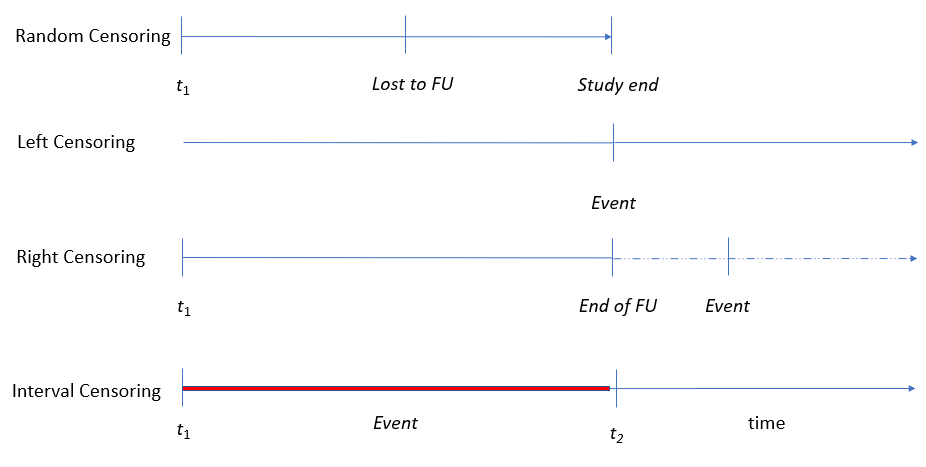
\includegraphics[width=1\linewidth]{figures/censoring}

\end{frame}

\begin{frame}{Infromative Censoring}
\protect\hypertarget{infromative-censoring}{}

The case where survival time is dependent with whatever causes the
censoring. Example: A patient in a community study is censored because
they are hospitalized (hospitalization indicates severity)

In most of the examples throughout we will make the assumption of
non-informative censoring

\end{frame}

\begin{frame}{What is survival analysis}
\protect\hypertarget{what-is-survival-analysis}{}

\begin{itemize}
\tightlist
\item
  Set of statistical methods that can handle:

  \begin{itemize}
  \tightlist
  \item
    Data skewness
  \item
    Censoring
  \item
    (Time-dependent) Covariates
  \item
    State transition processes
  \item
    Recurrent events
  \item
    The expectation of cure
  \end{itemize}
\item
  Used for both inference and extrapolation
\end{itemize}

\end{frame}

\begin{frame}{Key Concepts in survival analysis}
\protect\hypertarget{key-concepts-in-survival-analysis}{}

\begin{itemize}
\item
  survival to time \(T\): the random variable capturing time since the
  beginning of the event.
\item
  Survival: the probability of not experiencing an event unit some time
  \(t\) \(S(t) = Pr(T >t) = 1- Pr(T \leq t)\)
\item
  Cumulative density function:
\end{itemize}

\(F(t) = Pr(T \leq t)\)

\(F(t) = 1 - S(t)\)

\begin{itemize}
\tightlist
\item
  Hazard function (the instantaneous rate of the event):
  \(h(t) = \lim_{\delta t \rightarrow 0}\frac{1}{\delta t} \frac{ F(t + \delta t) - F(t)}{S(t)}\)
\end{itemize}

turns out \(h(t) = \frac{f(t)}{S(t)}\)

\begin{itemize}
\tightlist
\item
  Cumulative hazard \(H(t) \int^t_0 {h(x)dx}\)
\end{itemize}

as well as \(S(t) = e^{-H(t)}\)

\end{frame}

\begin{frame}{Example: the exponential distribution}
\protect\hypertarget{example-the-exponential-distribution}{}

\begin{itemize}
\item
  \(H(t) = \lambda t\)
\item
  \(S(t) = exp(-\lambda t)\)
\item
  \(f(t) = \lambda exp(-\lambda t)\)
\item
  Weibull , gamma, lognormal etc\ldots{}
\end{itemize}

\end{frame}

\begin{frame}{Some shapes of hazards}
\protect\hypertarget{some-shapes-of-hazards}{}

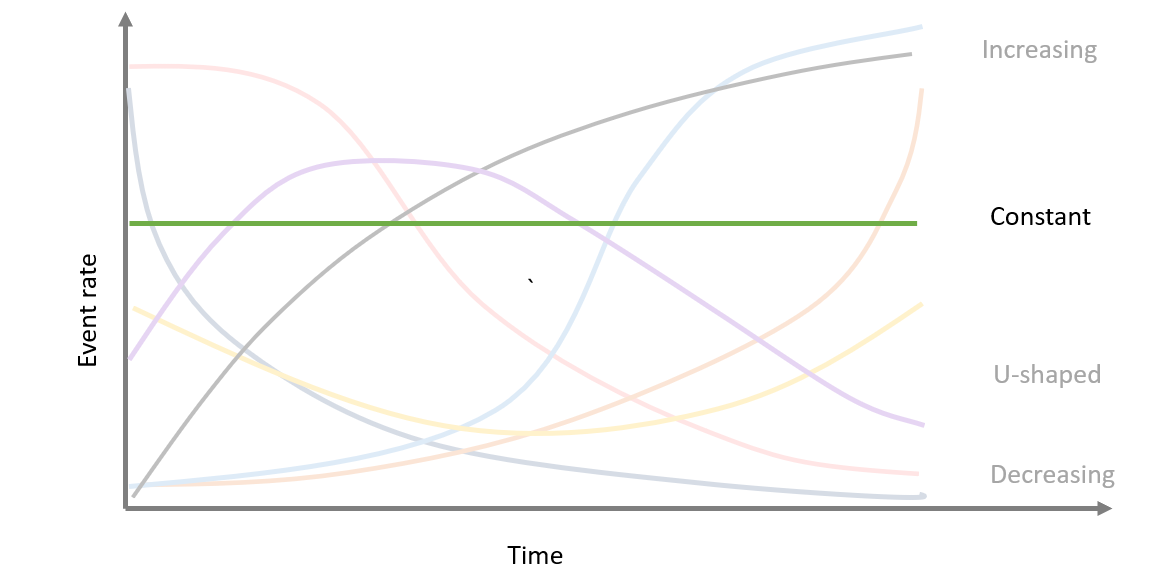
\includegraphics[width=1\linewidth]{figures/hazards}

\end{frame}

\begin{frame}{common distributions and hazard shapes}
\protect\hypertarget{common-distributions-and-hazard-shapes}{}

\begin{itemize}
\tightlist
\item
  Exponential:constant hazard
\item
  Weibull: hazard monotonically increases/decreases
\item
  Gompertz: hazard monotonically increases/decreases, but the rate of
  change is exponential
\item
  Log-logistic, log normal: hazard monotonically increases, and can then
  decrease
\end{itemize}

\end{frame}

\begin{frame}{Types of survival analysis models}
\protect\hypertarget{types-of-survival-analysis-models}{}

\begin{itemize}
\tightlist
\item
  Non-parametric models (e.g.~Kaplan Meier)
\item
  Semi-Parametric models (e.g.~Cox Proportional Hazard)
\item
  Parametric models (e.g.~Accelerated Failure Time)
\end{itemize}

\end{frame}

\begin{frame}{Non-Parametric models}
\protect\hypertarget{non-parametric-models}{}

\begin{itemize}
\tightlist
\item
  known as the ``product-limit'' estimator. The most used survival
  analysis method
\item
  makes no parametric assumption on the data
\end{itemize}

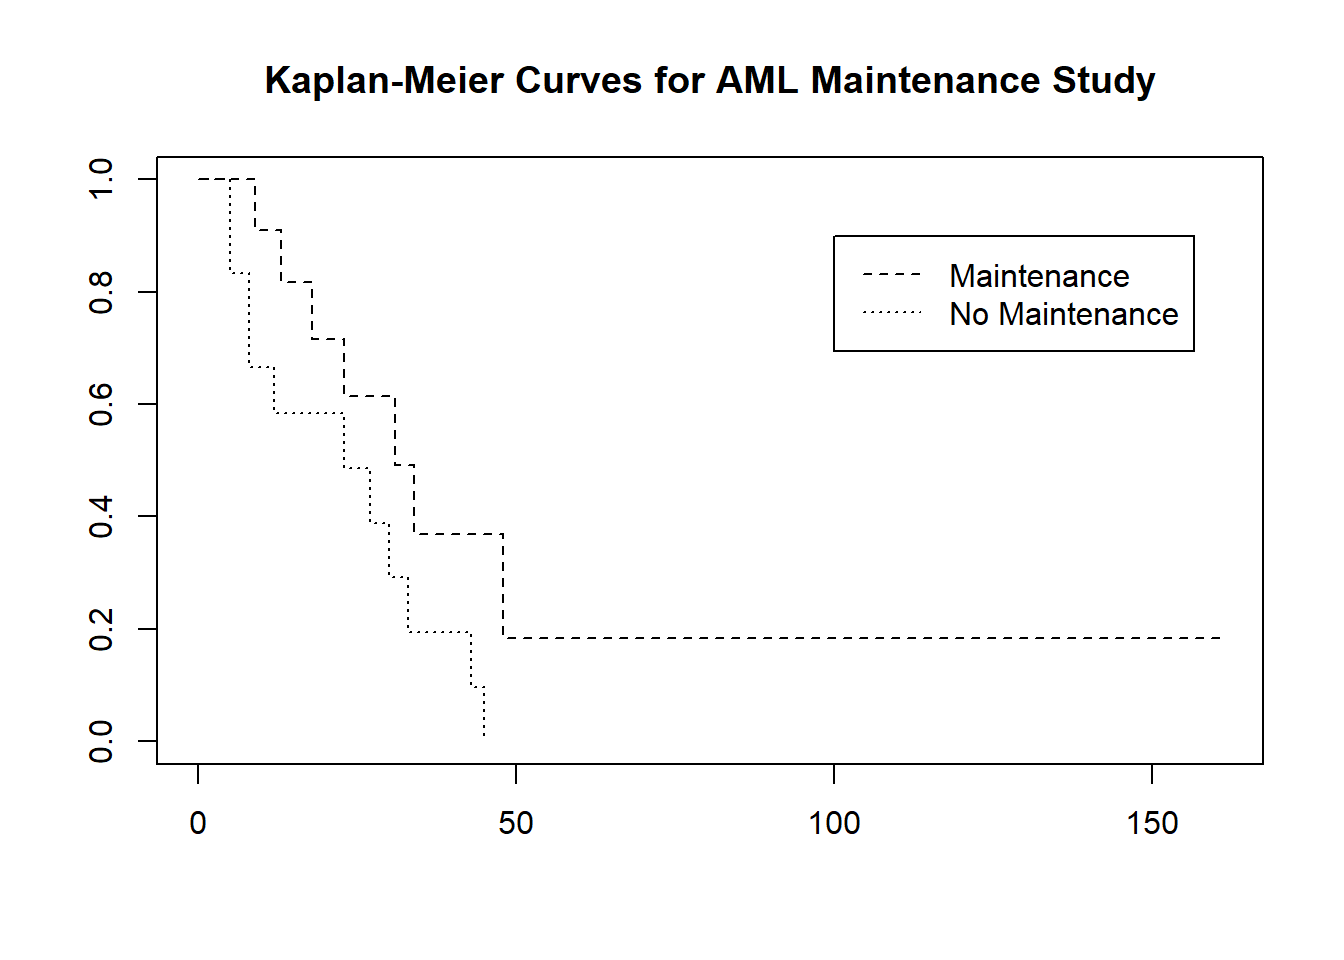
\includegraphics[width=1\linewidth]{ZIN_surv_files/figure-beamer/unnamed-chunk-3-1}

\end{frame}

\begin{frame}{Non-Parametric models}
\protect\hypertarget{non-parametric-models-1}{}

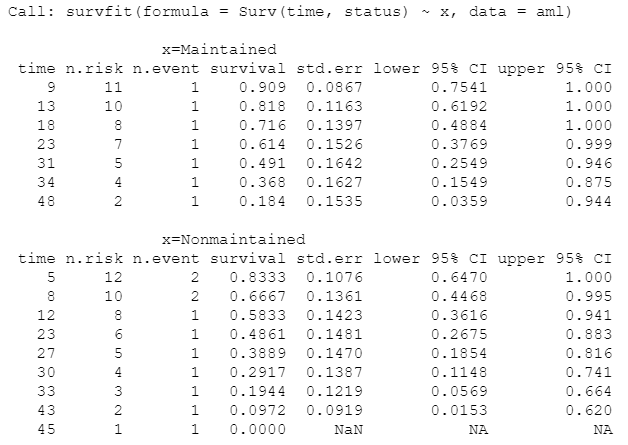
\includegraphics[width=1\linewidth]{figures/leukemia.surv_output}

\end{frame}

\begin{frame}{Non-Parametric models - testing}
\protect\hypertarget{non-parametric-models---testing}{}

\begin{itemize}
\item
  We can use a non parametric test to understand if group A lives longer
  than group B
\item
  long-rank test: is the difference in survival times statistically
  different?
\item
  relying on a \(\chi^2\) distribution
\end{itemize}

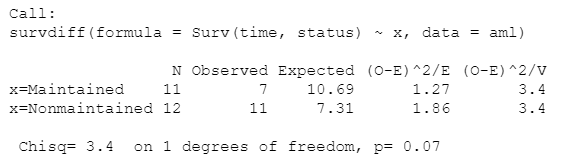
\includegraphics[width=1\linewidth]{figures/survdiff}

\end{frame}

\begin{frame}{Non-Parametric models}
\protect\hypertarget{non-parametric-models-2}{}

\begin{itemize}
\tightlist
\item
  Often, more intuitive to look at the results on the cumulative hazard
  rate
\item
  Nelson Aalen cumulative hazard is the most common non parametric
  estimator
\end{itemize}

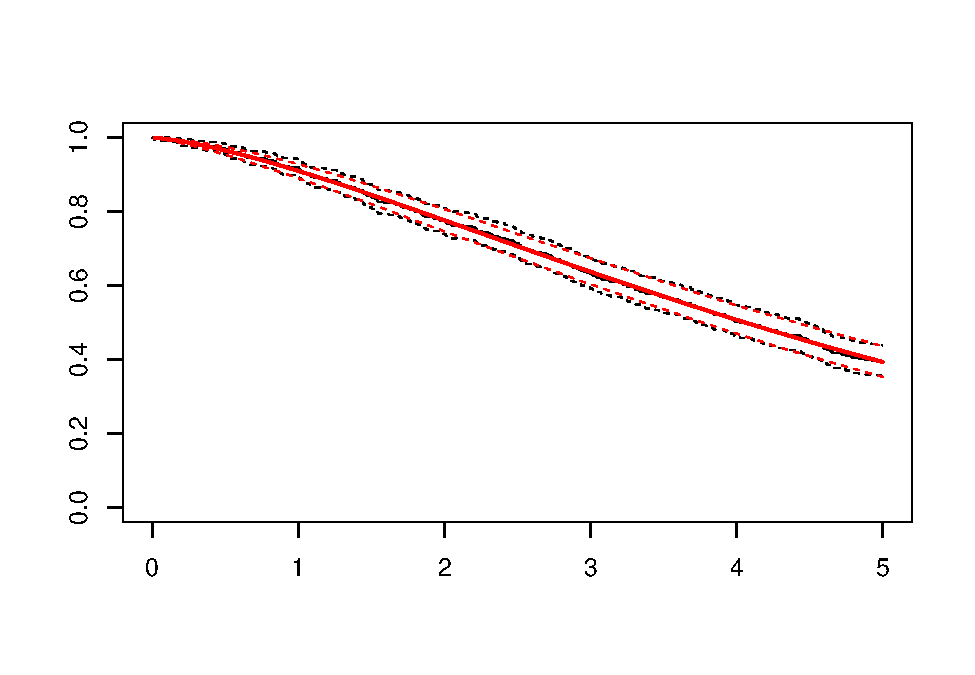
\includegraphics[width=1\linewidth]{ZIN_surv_files/figure-beamer/unnamed-chunk-8-1}

\end{frame}

\begin{frame}{Semi- Parametric models}
\protect\hypertarget{semi--parametric-models}{}

\begin{itemize}
\tightlist
\item
  Cox proportional hazard model

  \begin{itemize}
  \tightlist
  \item
    Hazard: the instantaneous risk of an event at time \(t\),
    conditional on survival to that time.
  \end{itemize}
\item
  Semi:

  \begin{itemize}
  \tightlist
  \item
    Baseline hazard modelled non parametrically (i.e effect of time)
  \item
    Covariate effects ( \(\beta\) 's) modelled parametrically (like in a
    regression model)
  \end{itemize}
\end{itemize}

\(h(t) = h_0(t)exp(X\beta)\) where \(h_0(t)\) is estimated
non-parametrically

Notice that the effect of the covariates is proportional on the baseline
hazard..(that's why ``proportional hazard'' model)

\end{frame}

\begin{frame}{The assumption of proportional hazards}
\protect\hypertarget{the-assumption-of-proportional-hazards}{}

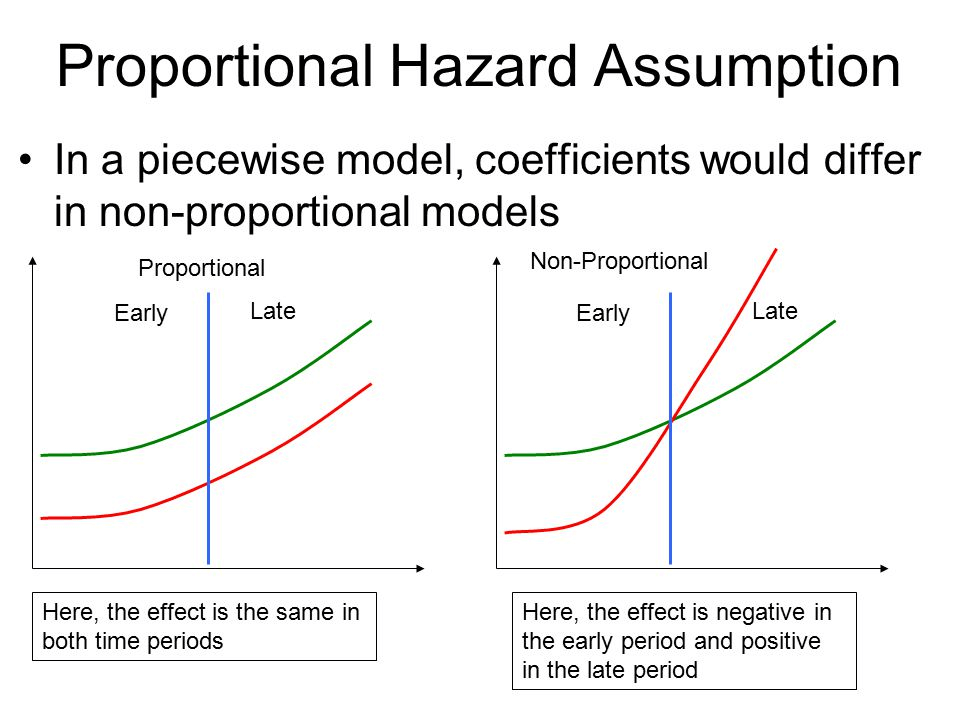
\includegraphics[width=1\linewidth]{figures/Churn}
source:\url{https://altis.com.au/a-crash-course-in-survival-analysis-customer-churn-part-iii/}

\end{frame}

\begin{frame}{Assessing the proportionality assumption}
\protect\hypertarget{assessing-the-proportionality-assumption}{}

The assumption can be assessed number of ways : visually

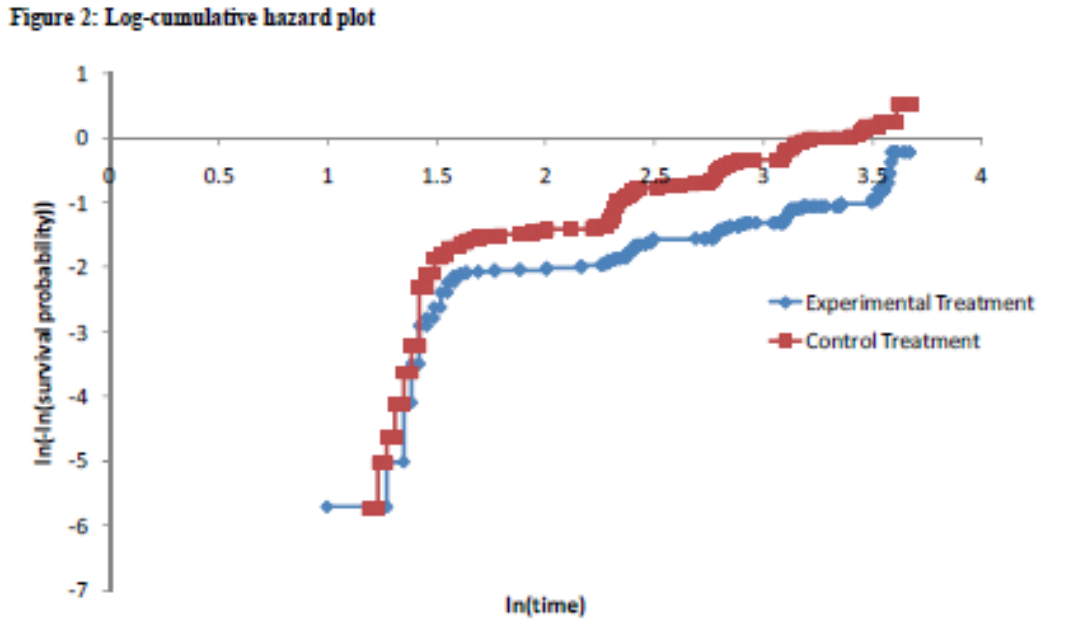
\includegraphics[width=1\linewidth]{figures/prop}
\url{http://nicedsu.org.uk/wp-content/uploads/2016/03/NICE-DSU-TSD-Survival-analysis.updated-March-2013.v2.pdf}

Testing the non-zero slope of the Schoenfeld residuals

\end{frame}

\begin{frame}{Fully Parametric models (Accelerated Failure Time models)}
\protect\hypertarget{fully-parametric-models-accelerated-failure-time-models}{}

\begin{itemize}
\tightlist
\item
  Usually model time-to-event directly rather than hazard
\item
  Resemble a regression model but can capture censoring
\item
  Fit a distribution to the (observed) time-to-event data

  \begin{itemize}
  \tightlist
  \item
    1 parameter : exponential
  \item
    2 parameter : Weibull, lognormal, gamma etc
  \item
    3, 4 parameter: Gen.~gamma , Gen F etc
  \end{itemize}
\item
  Assumption that censored patients will follow similar patterns to the
  observed.
\item
  Temporal extrapolation possible !
\end{itemize}

\end{frame}

\begin{frame}{AFT and covariates}
\protect\hypertarget{aft-and-covariates}{}

\begin{itemize}
\tightlist
\item
  We can incorporate covariates in a sort of similar way as we would do
  in a linear regression model
  \(log(T) = \beta_0 + X\beta_1 + \epsilon\)
\end{itemize}

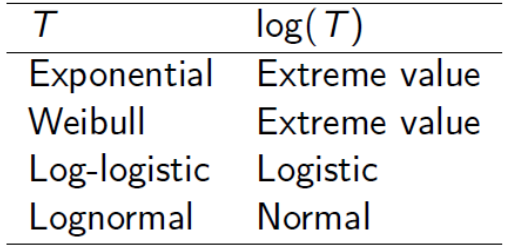
\includegraphics[width=1\linewidth]{figures/aft}

\end{frame}

\begin{frame}{Choosing the ``right'' distribution}
\protect\hypertarget{choosing-the-right-distribution}{}

\begin{itemize}
\tightlist
\item
  Statistical considerations of goodness-of-fit
\item
  Clinical plausibility

  \begin{itemize}
  \tightlist
  \item
    in-sample
  \item
    extrapolations
  \item
    out-of-sample
  \end{itemize}
\end{itemize}

\end{frame}

\begin{frame}{Goodness of fit metrics}
\protect\hypertarget{goodness-of-fit-metrics}{}

\begin{itemize}
\item
  Likelihood based metrics
\item
  Akaike Information Criterion (AIC)
\item
  Bayesian Information Criterion (BIC)
\item
  Performance based metrics
\item
  Sensitivity , Specificity
\item
  (time dependent) Receiver Operating characteristic (ROC) curve
\item
  Area Under the Curve (AUC)
\item
  c- statistic
\end{itemize}

\end{frame}

\begin{frame}{Choosing the ``right'' distribution}
\protect\hypertarget{choosing-the-right-distribution-1}{}

\begin{itemize}
\tightlist
\item
  NICE Decision Support Unit
\item
  Latimer et al 2011 : Survival Analysis For Economic Evaluations
  Alongside Clinical Trials - Extrapolation with Patient-Level Data

  \begin{itemize}
  \tightlist
  \item
    \textbf{Survival Model Selection Process algorithm}:

    \begin{itemize}
    \tightlist
    \item
      \emph{recommendations for how survival analysis can be undertaken
      more systematically. This involves fitting and testing a range of
      survival models and comparing these based upon internal validity
      (how well they fit to the observed trial data) and external
      validity (how plausible their extrapolated portions are)}
    \end{itemize}
  \end{itemize}
\end{itemize}

\end{frame}

\begin{frame}{Choosing the ``right'' distribution}
\protect\hypertarget{choosing-the-right-distribution-2}{}

Latimer et al 2011 (DSU 14)

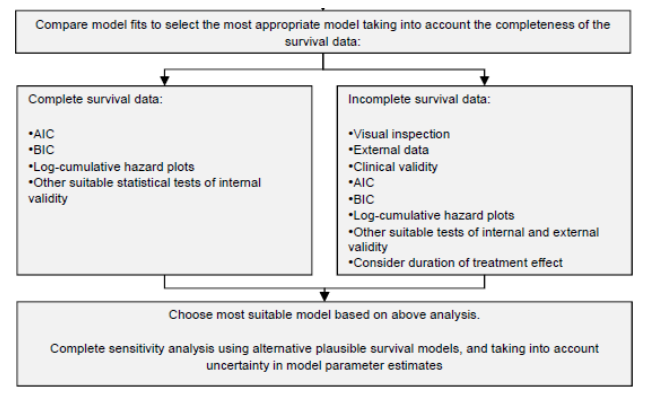
\includegraphics[width=1\linewidth]{figures/goflatimer}

\end{frame}

\begin{frame}{Flexible Survival models}
\protect\hypertarget{flexible-survival-models}{}

\begin{itemize}
\tightlist
\item
  Multi - parameter distributions

  \begin{itemize}
  \tightlist
  \item
    Generalized Gamma
  \item
    Generalized F
  \item
    Data hungry - possibiliy of overfitting\\
  \item
    Hypothesis testing possible
  \end{itemize}
\end{itemize}

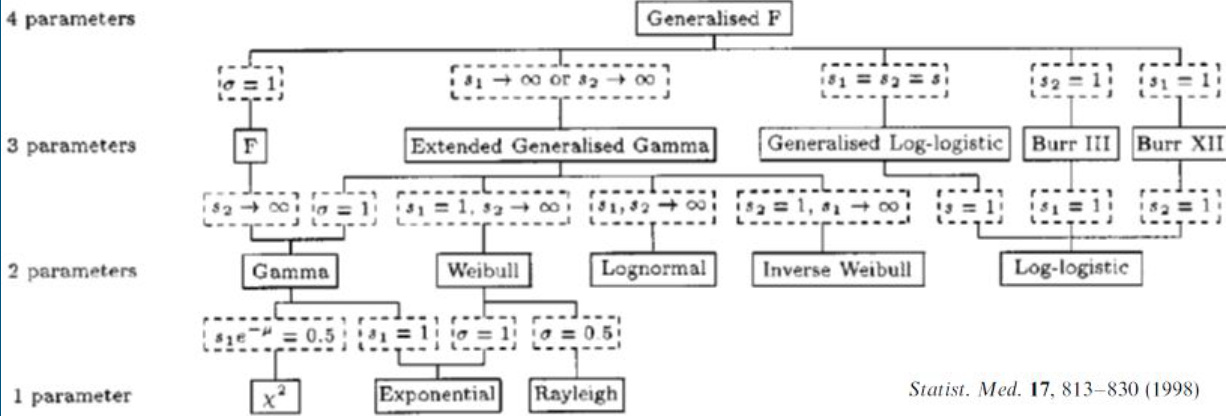
\includegraphics[width=1\linewidth]{figures/genf}

\end{frame}

\begin{frame}{Spline Survival models}
\protect\hypertarget{spline-survival-models}{}

\begin{itemize}
\tightlist
\item
  Survival models where the underlying hazard of an event is modelled as
  a smooth, piecewise polynomial function of time.
\item
  Extrapolation of hazard possible
\item
  Non-linear relation of time and hazard
\item
  Conventionally \emph{knots} are evenly spread on the (log)-time axis
\item
  Overfitting with too many knots possible -sensitivity analysis
\item
  AIC, BIC valid GoF tests
\item
  TSD 2020
\end{itemize}

\end{frame}

\begin{frame}{Spline Survival models}
\protect\hypertarget{spline-survival-models-1}{}

Gibson et al (Pharmacoeconomics, 2017)

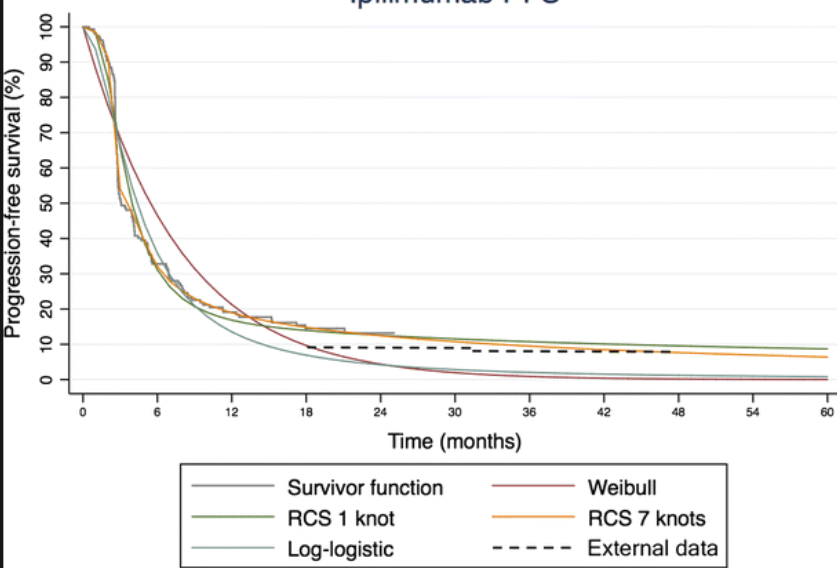
\includegraphics[width=1\linewidth]{figures/flexsurv}

\end{frame}

\begin{frame}{Spline Survival models}
\protect\hypertarget{spline-survival-models-2}{}

From Gibson et al (Pharacoeconomcs, 2017)

\emph{Spline-based models using a limited number of knots can provide an
acceptable fit to trial data and generate extrapolated estimates
supported by longer term evidence, with results that are stable in
response to changes in knot placement.}

\end{frame}

\begin{frame}{Approaches in extrapolation}
\protect\hypertarget{approaches-in-extrapolation}{}

Modeler faced with more decisions: - Extrapolate using KM and ``fitted''
tails - Extrapolate using the fitted curve

\begin{itemize}
\tightlist
\item
  Fit seperate curves to the data
\item
  Extrapolate treatment effect as relative
\item
  What is the behaviour of the relative effect post trial?
\item
  Regardless of the approach, the implied (observed or predicted)
  treatment effect should be presented
\end{itemize}

\end{frame}

\begin{frame}{Approaches in extrapolation}
\protect\hypertarget{approaches-in-extrapolation-1}{}


\includegraphics[width=1\linewidth]{figures/endmeans}

\end{frame}

\begin{frame}{Approaches in extrapolation}
\protect\hypertarget{approaches-in-extrapolation-2}{}

\begin{itemize}
\tightlist
\item
  Extrapolate using KM and ``fitted'' tails
\end{itemize}

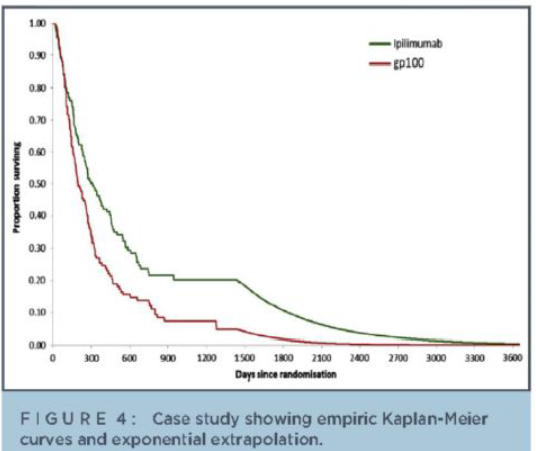
\includegraphics[width=1\linewidth]{figures/figure4means}

\end{frame}

\begin{frame}

\begin{itemize}
\tightlist
\item
  Extrapolate using the fitted curve
\end{itemize}

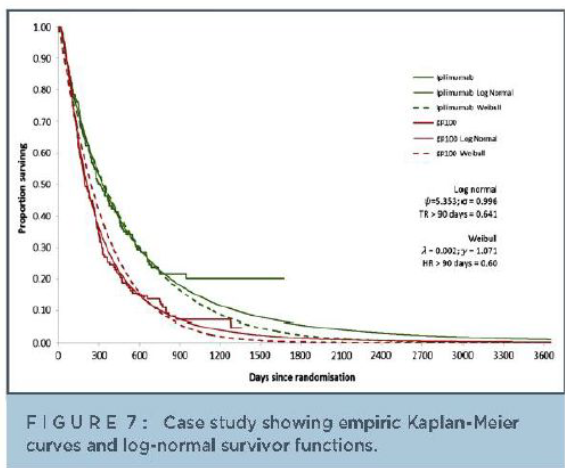
\includegraphics[width=1\linewidth]{figures/figure7means}

\end{frame}

\begin{frame}{Extrapolating a relative treatment effect}
\protect\hypertarget{extrapolating-a-relative-treatment-effect}{}

Drummond, et al (2015). Methods for the economic evaluation of health
care programmes. Oxford university press.

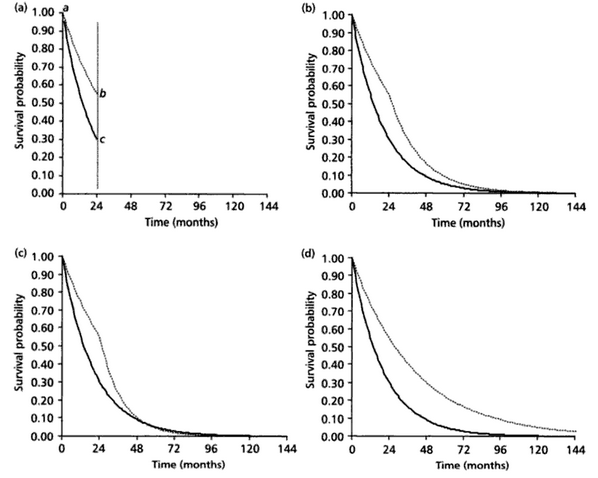
\includegraphics[width=0.6\linewidth]{figures/drummond}

\end{frame}

\end{document}
